The final evaluation of the project involved assessing the performance of the ensemble model on the test set, which was 20\% of the provided data. The final score was 0.498, consistent with the scores achieved in the Kaggle competition, suggesting a representative outcome.

\subsubsection*{Error distribution}
\begin{figure}[H]
    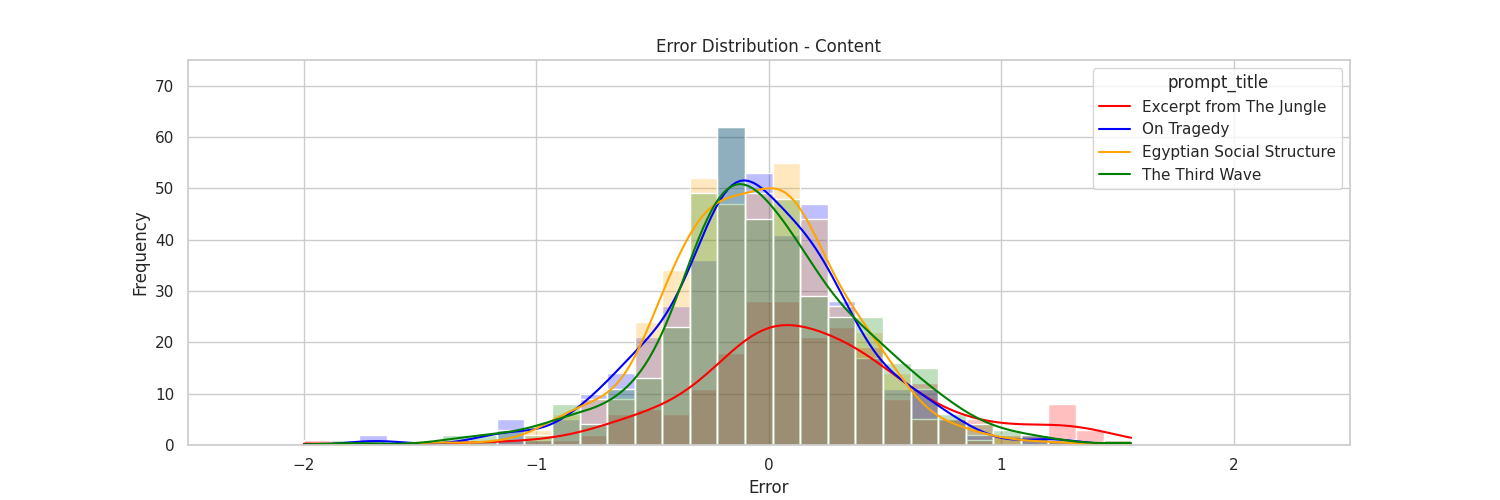
\includegraphics[keepaspectratio, width=\textwidth]{error_distribution_content.png}
    \caption{Error Distribution - Content}
    \label{fig:error_distribution_content}
\end{figure}
\begin{figure}[H]
    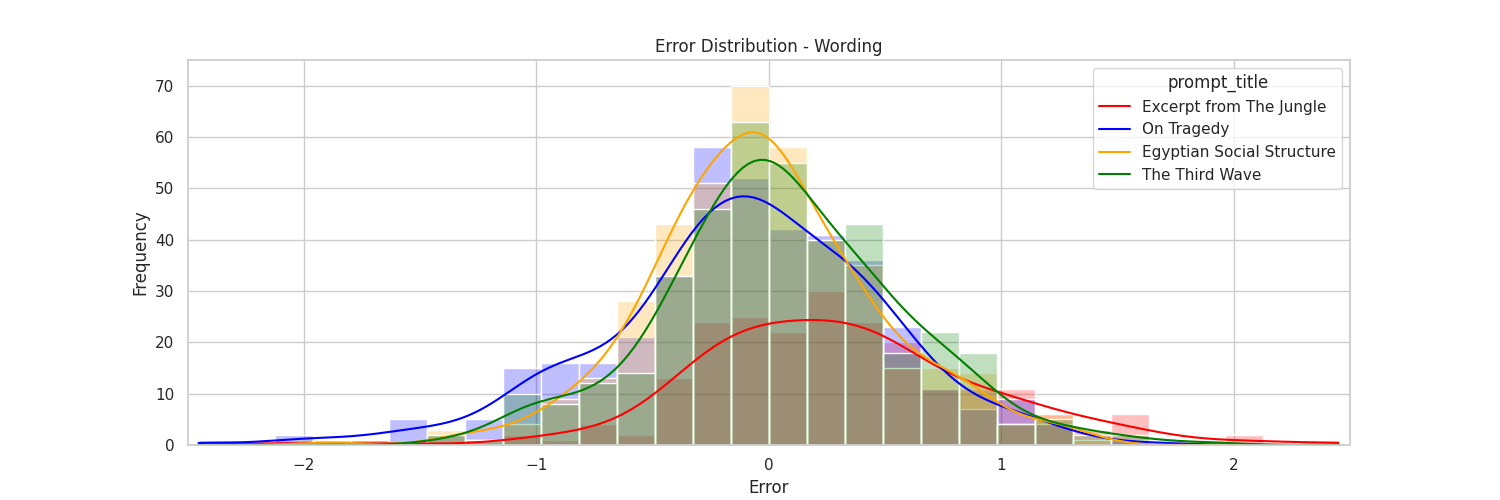
\includegraphics[keepaspectratio, width=\textwidth]{error_distribution_wording.png}
    \caption{Error Distribution - Wording}
    \label{fig:error_distribution_wording}
\end{figure}
The analysis of the error distribution for content and wording scores, as illustrated in Figures \ref{fig:error_distribution_content} and \ref{fig:error_distribution_wording}, 
reveals a gaussian distribution peak around zero, with most errors being smaller than 1. This suggests that the model's errors are generally small in magnitude. The even distribution also shows that the model does not tend to predict to high nor too low.

\subsubsection*{Mean absolute error}

\begin{figure}[H]
    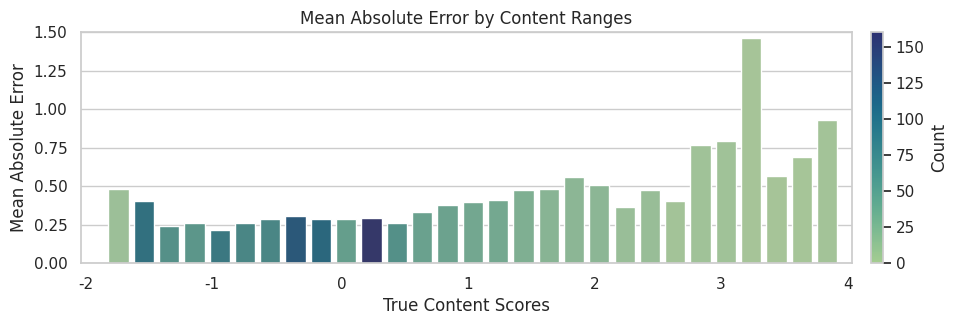
\includegraphics[keepaspectratio, width=\textwidth]{mean_absolute_error_content.png}
    \caption{Mean Absolute Error - Content}
    \label{fig:mean_absolute_error_content}
\end{figure}
\begin{figure}[H]
    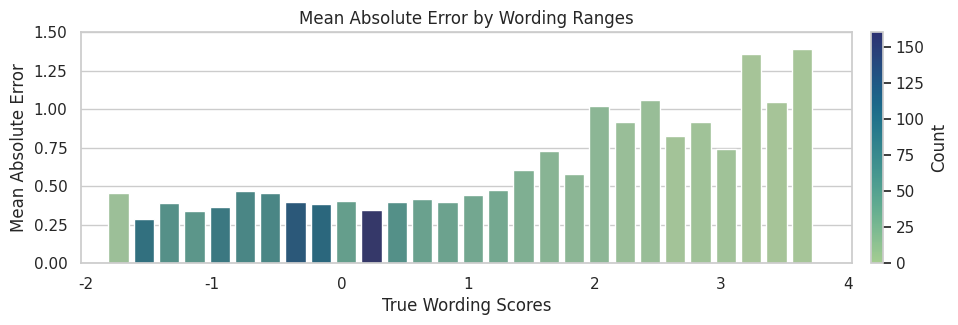
\includegraphics[keepaspectratio, width=\textwidth]{mean_absolute_error_wording.png}
    \caption{Mean Absolute Error - Wording}
    \label{fig:mean_absolute_error_wording}
\end{figure}
Displayed above are plots illustrating the \gls{mae} for the true content and wording scores. (Figure~\ref{fig:mean_absolute_error_content} and Figure~\ref{fig:mean_absolute_error_wording}) These plots use color intensity to represent data density: lighter shades indicate less training data in the dataset.
These plots reveal a tendency for higher \glspl{mae} in areas with lighter colors, suggesting that the model has difficulties with less frequent data. It can be inferred that an increase in data quantity within these lighter ranges would likely enhance the models performance.